% GNUPLOT: LaTeX picture with Postscript
\begingroup
  \makeatletter
  \providecommand\color[2][]{%
    \GenericError{(gnuplot) \space\space\space\@spaces}{%
      Package color not loaded in conjunction with
      terminal option `colourtext'%
    }{See the gnuplot documentation for explanation.%
    }{Either use 'blacktext' in gnuplot or load the package
      color.sty in LaTeX.}%
    \renewcommand\color[2][]{}%
  }%
  \providecommand\includegraphics[2][]{%
    \GenericError{(gnuplot) \space\space\space\@spaces}{%
      Package graphicx or graphics not loaded%
    }{See the gnuplot documentation for explanation.%
    }{The gnuplot epslatex terminal needs graphicx.sty or graphics.sty.}%
    \renewcommand\includegraphics[2][]{}%
  }%
  \providecommand\rotatebox[2]{#2}%
  \@ifundefined{ifGPcolor}{%
    \newif\ifGPcolor
    \GPcolortrue
  }{}%
  \@ifundefined{ifGPblacktext}{%
    \newif\ifGPblacktext
    \GPblacktexttrue
  }{}%
  % define a \g@addto@macro without @ in the name:
  \let\gplgaddtomacro\g@addto@macro
  % define empty templates for all commands taking text:
  \gdef\gplbacktext{}%
  \gdef\gplfronttext{}%
  \makeatother
  \ifGPblacktext
    % no textcolor at all
    \def\colorrgb#1{}%
    \def\colorgray#1{}%
  \else
    % gray or color?
    \ifGPcolor
      \def\colorrgb#1{\color[rgb]{#1}}%
      \def\colorgray#1{\color[gray]{#1}}%
      \expandafter\def\csname LTw\endcsname{\color{white}}%
      \expandafter\def\csname LTb\endcsname{\color{black}}%
      \expandafter\def\csname LTa\endcsname{\color{black}}%
      \expandafter\def\csname LT0\endcsname{\color[rgb]{1,0,0}}%
      \expandafter\def\csname LT1\endcsname{\color[rgb]{0,1,0}}%
      \expandafter\def\csname LT2\endcsname{\color[rgb]{0,0,1}}%
      \expandafter\def\csname LT3\endcsname{\color[rgb]{1,0,1}}%
      \expandafter\def\csname LT4\endcsname{\color[rgb]{0,1,1}}%
      \expandafter\def\csname LT5\endcsname{\color[rgb]{1,1,0}}%
      \expandafter\def\csname LT6\endcsname{\color[rgb]{0,0,0}}%
      \expandafter\def\csname LT7\endcsname{\color[rgb]{1,0.3,0}}%
      \expandafter\def\csname LT8\endcsname{\color[rgb]{0.5,0.5,0.5}}%
    \else
      % gray
      \def\colorrgb#1{\color{black}}%
      \def\colorgray#1{\color[gray]{#1}}%
      \expandafter\def\csname LTw\endcsname{\color{white}}%
      \expandafter\def\csname LTb\endcsname{\color{black}}%
      \expandafter\def\csname LTa\endcsname{\color{black}}%
      \expandafter\def\csname LT0\endcsname{\color{black}}%
      \expandafter\def\csname LT1\endcsname{\color{black}}%
      \expandafter\def\csname LT2\endcsname{\color{black}}%
      \expandafter\def\csname LT3\endcsname{\color{black}}%
      \expandafter\def\csname LT4\endcsname{\color{black}}%
      \expandafter\def\csname LT5\endcsname{\color{black}}%
      \expandafter\def\csname LT6\endcsname{\color{black}}%
      \expandafter\def\csname LT7\endcsname{\color{black}}%
      \expandafter\def\csname LT8\endcsname{\color{black}}%
    \fi
  \fi
    \setlength{\unitlength}{0.0500bp}%
    \ifx\gptboxheight\undefined%
      \newlength{\gptboxheight}%
      \newlength{\gptboxwidth}%
      \newsavebox{\gptboxtext}%
    \fi%
    \setlength{\fboxrule}{0.5pt}%
    \setlength{\fboxsep}{1pt}%
\begin{picture}(7200.00,5040.00)%
    \gplgaddtomacro\gplbacktext{%
      \csname LTb\endcsname%%
      \put(849,1039){\makebox(0,0)[r]{\strut{}$10^{-10}$}}%
      \csname LTb\endcsname%%
      \put(849,1928){\makebox(0,0)[r]{\strut{}$10^{-8}$}}%
      \csname LTb\endcsname%%
      \put(849,2817){\makebox(0,0)[r]{\strut{}$10^{-6}$}}%
      \csname LTb\endcsname%%
      \put(849,3706){\makebox(0,0)[r]{\strut{}$10^{-4}$}}%
      \csname LTb\endcsname%%
      \put(849,4595){\makebox(0,0)[r]{\strut{}$10^{-2}$}}%
      \csname LTb\endcsname%%
      \put(2844,409){\makebox(0,0){\strut{}0.05}}%
      \csname LTb\endcsname%%
      \put(5552,409){\makebox(0,0){\strut{}0.5}}%
      \csname LTb\endcsname%%
      \put(7183,409){\makebox(0,0){\strut{}2}}%
      \csname LTb\endcsname%%
      \put(951,409){\makebox(0,0){\strut{}0.01}}%
      \csname LTb\endcsname%%
      \put(3659,409){\makebox(0,0){\strut{}0.1}}%
      \csname LTb\endcsname%%
      \put(6368,409){\makebox(0,0){\strut{}1}}%
    }%
    \gplgaddtomacro\gplfronttext{%
      \csname LTb\endcsname%%
      \put(153,2817){\rotatebox{-270}{\makebox(0,0){\strut{}$|U_{e N}|^2$}}}%
      \csname LTb\endcsname%%
      \put(4067,130){\makebox(0,0){\strut{}Mass (GeV)}}%
      \csname LTb\endcsname%%
      \put(4151,3713){\makebox(0,0)[l]{\strut{}FASER}}%
      \csname LTb\endcsname%%
      \put(4151,3917){\makebox(0,0)[l]{\strut{}MATHUSLA}}%
      \csname LTb\endcsname%%
      \put(4151,4121){\makebox(0,0)[l]{\strut{}NA62}}%
      \csname LTb\endcsname%%
      \put(4151,4325){\makebox(0,0)[l]{\strut{}SHiP}}%
      \csname LTb\endcsname%%
      \put(4151,4529){\makebox(0,0)[l]{\strut{}SBND}}%
      \csname LTb\endcsname%%
      \put(4151,4733){\makebox(0,0)[l]{\strut{}DUNE}}%
      \csname LTb\endcsname%%
      \put(4151,4937){\makebox(0,0)[l]{\strut{} }}%
      \csname LTb\endcsname%%
      \put(849,1039){\makebox(0,0)[r]{\strut{}$10^{-10}$}}%
      \csname LTb\endcsname%%
      \put(849,1928){\makebox(0,0)[r]{\strut{}$10^{-8}$}}%
      \csname LTb\endcsname%%
      \put(849,2817){\makebox(0,0)[r]{\strut{}$10^{-6}$}}%
      \csname LTb\endcsname%%
      \put(849,3706){\makebox(0,0)[r]{\strut{}$10^{-4}$}}%
      \csname LTb\endcsname%%
      \put(849,4595){\makebox(0,0)[r]{\strut{}$10^{-2}$}}%
      \csname LTb\endcsname%%
      \put(2844,409){\makebox(0,0){\strut{}0.05}}%
      \csname LTb\endcsname%%
      \put(5552,409){\makebox(0,0){\strut{}0.5}}%
      \csname LTb\endcsname%%
      \put(7183,409){\makebox(0,0){\strut{}2}}%
      \csname LTb\endcsname%%
      \put(951,409){\makebox(0,0){\strut{}0.01}}%
      \csname LTb\endcsname%%
      \put(3659,409){\makebox(0,0){\strut{}0.1}}%
      \csname LTb\endcsname%%
      \put(6368,409){\makebox(0,0){\strut{}1}}%
      \csname LTb\endcsname%%
      \put(2844,4284){\makebox(0,0){\strut{}\textbf{Excluded}}}%
      \csname LTb\endcsname%%
      \put(1766,996){\makebox(0,0){\strut{}\textbf{Majorana state}}}%
      \csname LTb\endcsname%%
      \put(1766,2373){\makebox(0,0){\strut{}\textbf{\shortstack{Pseudo-Dirac\\pair}}}}%
      \csname LTb\endcsname%%
      \put(2844,1484){\rotatebox{-5}{\makebox(0,0){\strut{}\textbf{Type I}}}}%
    }%
    \gplbacktext
    \put(0,0){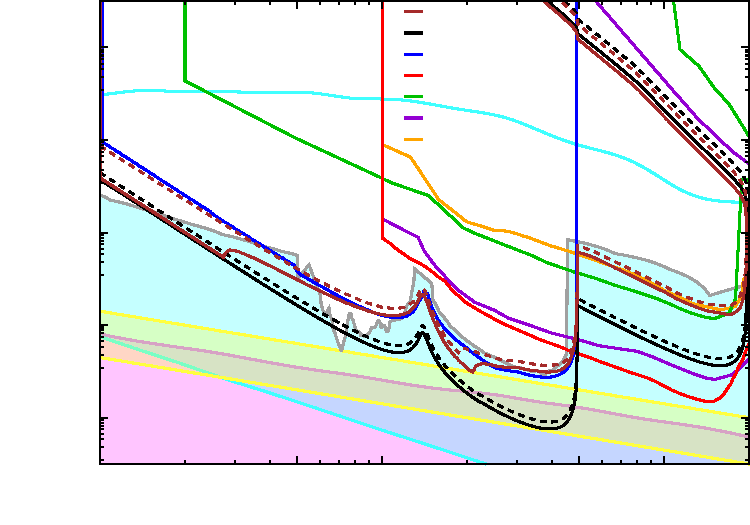
\includegraphics{pics/DUNE_HNL_E_real}}%
    \gplfronttext
  \end{picture}%
\endgroup
